% Revised manuscript prepared from formatting-instructions-latex-2024.tex
% and the frozen experimental artifacts in hardware_results/results/.
\documentclass[letterpaper]{article} % DO NOT CHANGE THIS
\usepackage{aaai24}  % DO NOT CHANGE THIS
\usepackage{times}  % DO NOT CHANGE THIS
\usepackage{helvet}  % DO NOT CHANGE THIS
\usepackage{courier}  % DO NOT CHANGE THIS
\usepackage[hyphens]{url}  % DO NOT CHANGE THIS
\usepackage{graphicx} % DO NOT CHANGE THIS
\urlstyle{rm} % DO NOT CHANGE THIS
\def\UrlFont{\rm}  % DO NOT CHANGE THIS
\usepackage{natbib}  % DO NOT CHANGE THIS AND DO NOT ADD ANY OPTIONS TO IT
\usepackage{caption} % DO NOT CHANGE THIS AND DO NOT ADD ANY OPTIONS TO IT
\usepackage{amsmath}
\usepackage{booktabs}
\frenchspacing  % DO NOT CHANGE THIS
\setlength{\pdfpagewidth}{8.5in}  % DO NOT CHANGE THIS
\setlength{\pdfpageheight}{11in}  % DO NOT CHANGE THIS

\pdfinfo{
/TemplateVersion (2024.1)
}

\setcounter{secnumdepth}{0}

\title{Hardware-Measured Quantum Kernels for Malware Detection: Distortion and Classification Stability}
\author{
    Mary L. Cotrupi\textsuperscript{\rm 1}, Allison Aurilio\textsuperscript{\rm 2}, Sean Sanpietro\textsuperscript{\rm 3}, Fabiana Torres\textsuperscript{\rm 4}, Anwita Kasturi\textsuperscript{\rm 1}, Quinn Colognato\textsuperscript{\rm 1}, Brian Robert Callahan\textsuperscript{\rm 4}
}
\affiliations{
    \textsuperscript{\rm 1}Dept. of Computer Science, Rensselaer Polytechnic Institute, Troy, NY 12180-3590 USA\\
    \textsuperscript{\rm 2}Dept. of Electrical and Computer Engineering, The College of New Jersey, 2000 Pennington Road, Ewing, NJ 08618-1100 USA\\
    \textsuperscript{\rm 3}Dept. of Computer Science, Misericordia University, 301 Lake Street, Dallas, PA 18612-7752 USA\\
    \textsuperscript{\rm 4}Dept. of Computer Science and Software Engineering, Monmouth University, 400 Cedar Avenue, West Long Branch, NJ 07764-1828 USA\\
    cotrum@rpi.edu, aurilia2@tcnj.edu, ssanpiet@misercordia.edu, s1378769@monmouth.edu, kastua@rpi.edu, cologq@rpi.edu, bcallaha@monmouth.edu
}

\begin{document}

\maketitle

\begin{abstract}
Quantum machine learning (QML) has been proposed for malware detection, but much of the literature remains simulator based, leaving the effect of real device noise insufficiently characterized. We study whether execution-induced changes in quantum-kernel geometry translate into changes in downstream classification. Across four malware datasets, six dataset--representation configurations, and three repeated held-out splits, we evaluated a fidelity-kernel support vector classifier using exact statevectors, ideal 512-shot Aer simulation, backend-derived noisy 512-shot Aer simulation, and 512-shot execution on \texttt{ibm\_rensselaer}. Exact evaluation establishes the reference kernel, while ideal Aer isolates finite-shot estimation before modeled and measured device effects are introduced. Mean hardware relative Frobenius error was 0.111--0.114 for four-qubit configurations, 0.441 at eight qubits, and 0.479 at ten qubits. Nevertheless, hardware-minus-exact balanced accuracy ranged only from $-1.67$ to $+1.25$ percentage points. Paired confidence intervals included zero, and no hardware-versus-exact prediction comparison was significant after Holm adjustment. Because no practical-equivalence margin was prespecified, these results show empirical classification stability under the tested conditions, not formal equivalence. Principal component analysis (PCA) reduced circuit cost and hardware distortion but caused dataset-dependent accuracy losses, including 10.0 points for CLaMP. Matched classical models remained competitive; no quantum advantage was demonstrated.
\end{abstract}

\section{Introduction}

Quantum computing offers new methods for representing and processing data and is increasingly being studied for defensive cybersecurity applications. At the same time, the practical value of quantum machine learning depends on behavior on noisy, presently available hardware rather than only under ideal simulation.

Malicious binaries, more commonly called malware, are a persistent threat. Malware detection remains difficult both in theory~\cite{cohen1987computer} and in practice~\cite{pachhala}. Prior QML studies have reported preliminary results for cybersecurity tasks such as malicious network-traffic classification~\cite{cotrupi}, motivating further study of where quantum methods may be useful to practitioners.

Many QML malware experiments have been conducted only in simulation. A simulated classifier can validate an implementation, but it cannot fully represent finite sampling, device-specific errors, calibration drift, and the cumulative effects of transpiled circuit execution. We therefore examine a controlled execution ladder:
\[
\text{exact statevector}
\rightarrow \text{ideal shot-based Aer}
\rightarrow \text{backend-noise Aer}
\rightarrow \text{IBM hardware}.
\]
Including both exact and ideal-Aer conditions is deliberate: their difference isolates finite-shot estimation of a transpiled circuit before modeled device noise is added.

This study asks two related questions. First, how do finite sampling, a backend-derived noise model, and real hardware alter quantum-kernel geometry and malware-classification performance? Second, how does four-component PCA trade predictive information for lower circuit width and noise exposure? Our contributions are (1) a real-hardware evaluation spanning four malware datasets and six dataset--representation configurations and (2) a reproducible comparison of numerical kernel distortion with downstream classifier behavior. Matched linear and radial-basis-function (RBF) support vector classifiers provide classical context rather than an optimized quantum-advantage benchmark.

The central finding is that hardware substantially distorted the wider measured kernels, yet the observed balanced-accuracy changes relative to exact kernels remained small. We describe this as empirical stability within the tested workflow. We do not claim that hardware and exact execution are statistically equivalent, that quantum models outperform optimized classical models, or that the experiment demonstrates a speed or energy advantage.

\section{Background}

The intersection of quantum computing and applied cybersecurity is developing into an active area of study. Recent work, for example, has explored quantum methods for Distributed Denial-of-Service traffic analysis~\cite{cogburn2026hardwareawareqaoahoneypottraffic}.

Within malware detection, prior work has compared classical, hybrid, and quantum models for Android malware. Purely quantum approaches were competitive on some small datasets but did not scale to the largest evaluated data, where classical methods remained stronger~\cite{mercaldo2022towards}. Other work compared a quantum multilayer perceptron with a quantum convolutional neural network, reporting a tradeoff between predictive accuracy and training efficiency~\cite{11249907}.

Several malware studies either do not identify a real-hardware execution environment~\cite{joshi2025quantumaialgorithmdevelopment} or explicitly report simulator-only experiments~\cite{10.1145/3538969.3543816,mercaldo2022towards,11249907,10.1145/3696673.3723063}. More recent studies have used real quantum hardware for malicious network-traffic detection~\cite{cotrupi}, supply-chain malware detection~\cite{11071553}, and comparisons between quantum support vector machines and quantum neural networks~\cite{10.1007/978-3-031-74643-7_19}. Some hardware studies also use malware data represented in the present corpus~\cite{11071553}.

A quantum-kernel classifier separates quantum representation from classical optimization. A parameterized feature map encodes each input into a quantum state, quantum execution estimates pairwise state fidelities, and a classical support vector classifier (SVC) fits the resulting precomputed kernel. This structure is useful for the present question because the same classifier and inputs can be held fixed while the kernel is measured under progressively more realistic execution conditions.

\section{Methodology}

\subsection{Study Design and Datasets}

We conducted a controlled comparison of exact, simulated, and hardware-measured quantum kernels for binary malware classification. Labels 0 and 1 denote benign and malware, respectively. The study comprised six dataset--representation configurations, three repeated held-out splits per configuration, and four quantum execution environments. CLaMP and the Malware and Benign Recognition (MBR) data were evaluated using both selected native features and a four-component PCA representation. CIC-YNU-IoTMal and EMBER2018 were evaluated with four components because their original feature spaces exceeded the hardware widths used in this study. MBR is our abbreviation for the Kaggle malware/benign collection published by Aashish.zzz~\cite{synthetic}; frozen artifact identifiers retain the earlier prefix \texttt{fabiana\_} for traceability.

\begin{table*}[t]
\centering
\small
\caption{Datasets and evaluated representations. Candidate-pool counts follow deterministic source sampling, where applicable, and removal of duplicate feature vectors.}
\label{tab:dataset-design}
\begin{tabular}{lp{2.75in}rrl}
\toprule
Dataset & Observation and predictors & Source rows & Candidate pool & Configuration(s) \\
\midrule
CLaMP & Windows PE file; 10 selected header fields & 5,184 & 4,040 & Native-10, PCA-4 \\
MBR & Windows PE file; 8 selected header fields & 1,156 & 895 & Native-8, PCA-4 \\
CIC-YNU-IoTMal & Sandbox activity record; 314 numeric SAR fields & 2,121,949 & 1,280 & PCA-4 \\
EMBER2018 & Windows PE file; 2,381-dimensional static vector & 799,912 & 1,200 & PCA-4 \\
\bottomrule
\end{tabular}
\end{table*}

CLaMP~\cite{clamp} contains static Windows Portable Executable (PE) metadata. We selected \texttt{NumberOfSections}, \texttt{Characteristics}, \texttt{Magic}, \texttt{MajorLinkerVersion}, \texttt{SizeOfCode}, \texttt{AddressOfEntryPoint}, \texttt{ImageBase}, \texttt{SizeOfImage}, \texttt{DllCharacteristics}, and \texttt{SizeOfStackReserve}. Its 5,184 source rows produced 4,040 unique, consistently labeled vectors: 2,275 benign and 1,765 malware.

MBR contains static PE metadata. We selected \texttt{SizeOfCode}, \texttt{SizeOfInitializedData}, \texttt{SizeOfUninitializedData}, \texttt{AddressOfEntryPoint}, \texttt{BaseOfData}, \texttt{ImageBase}, \texttt{NumberOfSections}, and \texttt{DllCharacteristics}. Its 1,156 source rows produced 895 unique, consistently labeled vectors: 546 benign and 349 malware.

CIC-YNU-IoTMal 2026~\cite{cic} contains Linux system-activity reports collected while benign and malicious Internet-of-Things binaries ran in ARM, MIPS, MIPSEL, and x86 sandboxes. We used the 314 numeric fields shared across the four architecture files and assigned label 1 whenever \texttt{MalwareFamily} was not \texttt{Benign}. We deterministically sampled 160 benign and 160 malicious candidates per architecture, producing a pool of 1,280 records balanced by class and architecture.

EMBER2018~\cite{ember2018} represents Windows PE files with 2,381 static features derived from byte and byte-entropy histograms, strings, general and header metadata, sections, imports, exports, and data directories. From the local 799,912-row vectorized release, we excluded raw label $-1$ (unlabeled) and deterministically selected 600 rows from each of labels 0 and 1.

Before splitting, complete selected feature vectors were hashed. Identical vectors carrying one label were represented once, while a group would have been excluded if the same vector carried conflicting labels. Duplicate filtering removed 1,144 CLaMP rows and 261 MBR rows; no conflicting-label group was found. Neither sampled CIC nor EMBER2018 contained duplicate complete feature vectors. Source identifiers, feature hashes, labels, source-file hashes, and selected indices were retained in the experimental artifacts.

\subsection{Repeated Holdouts and Preprocessing}

We generated three deterministic repeated holdouts using master seed 20,260,825 and split-specific training seeds 101, 204, and 303. Each split contained 80 training and 80 test observations, with 40 benign and 40 malware observations in each partition. Test observations were source-row disjoint across the three splits and were reserved before training samples were drawn; no training set contained any observation reserved for a test set. Training sets could overlap with one another, so the splits are repeated holdouts rather than independent experimental replicates. CIC partitions additionally contained 10 observations from each class--architecture stratum. Native and PCA configurations for CLaMP and MBR used the same source identifiers and labels within each split.

All preprocessing transformations were fitted only on the corresponding 80-row training partition and then applied to its test partition. Missing and infinite values were handled by median imputation. Native inputs were min--max scaled to $[0,1]$. For PCA inputs, imputed variables were standardized, transformed using full-SVD PCA fitted to the training data, reduced to four components, and then min--max scaled to $[0,1]$. Test coordinates outside the training range were clipped. The mean cumulative training variance represented by four components was 0.671 for CLaMP, 0.850 for MBR, 0.529 for CIC, and 0.343 for EMBER2018. Each transformed matrix was checked for finite values, and no transformed test vector exactly matched a training vector.

\subsection{Quantum Kernel and Execution Environments}

An $n$-qubit system has a $2^n$-dimensional Hilbert space. Here, each of $d$ input coordinates was assigned to one qubit, mapping the classical input to a quantum state in a $2^d$-dimensional Hilbert space; this dimensionality alone does not imply a computational advantage. We used Qiskit's \texttt{zz\_feature\_map}~\cite{qiskit2024} with two repetitions and linear entanglement. Defining
\[
|\phi(\mathbf{x})\rangle=U_{\phi}(\mathbf{x})|0^d\rangle,
\]
the fidelity kernel is
\begin{equation}
K(\mathbf{x},\mathbf{z})=
\left|\langle 0^d|U_{\phi}^{\dagger}(\mathbf{z})
U_{\phi}(\mathbf{x})|0^d\rangle\right|^2,
\label{eq:fidelity-kernel}
\end{equation}
where $d\in\{4,8,10\}$ is both the input dimension and the number of logical qubits.

The fidelity circuit applies $U_{\phi}(\mathbf{x})$ followed by $U_{\phi}^{\dagger}(\mathbf{z})$, measures every qubit, and estimates the kernel entry as the frequency of the all-zero outcome. We evaluated four environments: (1) exact statevector fidelity without sampling; (2) ideal Aer execution of the transpiled circuit with 512 shots; (3) 512-shot Aer execution with a backend-derived noise model; and (4) 512-shot execution on \texttt{ibm\_rensselaer}. Exact statevectors provide the reference geometry. Ideal Aer preserves the hardware-compatible circuit and finite-shot estimator without a noise model, allowing the next two stages to distinguish modeled and measured device effects.

The ideal-Aer, noisy-Aer, and hardware modes used the same fixed transpiled instruction-set circuit. Circuits were transpiled once against the \texttt{ibm\_rensselaer} target, including its coupling constraints, at optimization level 3 with transpiler seed 42. The resulting operations used \texttt{rz}, \texttt{sx}, \texttt{x}, and \texttt{cz} gates followed by measurement. The logical-to-physical layouts were $[116,106,105,115]$ at four qubits, $[114,104,105,106,116,117,107,97]$ at eight qubits, and $[103,104,114,115,105,106,116,117,107,97]$ at ten qubits. Active physical wires and their corresponding noise channels were relabeled densely for Aer without changing circuit operations.

The noisy-Aer model was constructed with Qiskit's \texttt{NoiseModel.from\_backend} from a serialized \texttt{ibm\_rensselaer} property snapshot captured during the August 26, 2026 campaign. It retained the backend-derived gate and readout-error channels for the active physical qubits. The dense model omitted the backend's custom delay-relaxation pass because the frozen circuits contained no delay instructions. The source noise model, reduced active-wire models, transpiled circuits, physical layouts, and a backend-property snapshot before every hardware submission were archived. Dynamical decoupling, gate twirling, measurement twirling, and measurement-error mitigation were not enabled.

For each condition, the symmetric training kernel required $80(79)/2=3,160$ off-diagonal circuit evaluations; the diagonal was set to one. The rectangular test kernel required $80\times80=6,400$ evaluations. Each shot-based condition therefore used 9,560 circuit evaluations and 4,894,720 shots.

\begin{table}[t]
  \centering
  \small
  \caption{Transpiled circuit resources for \texttt{ibm\_rensselaer}. Duration is the estimated duration of one transpiled fidelity circuit based on backend instruction timings, not total job or QPU usage.}
  \label{tab:circuit-resources}
  \begin{tabular}{rrrrr}
  \toprule
  Qubits & Depth & Size & CZ gates & Duration ($\mu$s) \\
  \midrule
  4  & 98  & 174 & 22 & 5.308 \\
  8  & 170 & 400 & 54 & 7.524 \\
  10 & 206 & 518 & 70 & 8.660 \\
  \bottomrule
  \end{tabular}
\end{table}

\subsection{Kernel Conditioning, Classification, and Metrics}

Finite-shot training kernels were first symmetrized as $K_s=(K+K^{T})/2$ and assigned a unit diagonal. We then eigendecomposed $K_s$, clipped every negative eigenvalue to zero, reconstructed the matrix, and normalized it to a unit diagonal. The same procedure was applied to exact training kernels for a matched analysis. Rectangular test kernels were neither symmetrized nor projected. A precomputed-kernel SVC with fixed $C=1$ was fitted to each conditioned training kernel~\cite{scholkopf2002,qiskit2024}.

Matched classical checks used linear and RBF SVCs with $C=1$ and, for RBF, \texttt{gamma=scale}. They received the same transformed inputs as the quantum method. No classifier or preprocessing hyperparameter was selected from test or hardware results. These fixed models were designed as controlled checks, not as optimized classical benchmarks.

The primary predictive endpoint was balanced accuracy, the mean of benign and malware recall. ROC AUC calculated from SVC decision scores was secondary. For execution mode $m$ and exact test kernel $K_e$, relative Frobenius error was
\begin{equation}
E_F(m)=\frac{\|K_m-K_e\|_F}{\|K_e\|_F}.
\label{eq:relative-frobenius}
\end{equation}
We also calculated Pearson correlation between the flattened test-kernel entries. Kernel-error calculations used the unprojected rectangular test kernels.

\subsection{Statistical Analysis}

Reported means and standard deviations are across three held-out splits. We formed 95\% bootstrap intervals from 10,000 replicates by resampling observations separately within each split and class and then averaging the three split metrics. For $\Delta=\mathrm{BA}_{\mathrm{hardware}}-\mathrm{BA}_{\mathrm{exact}}$, the same sampled observation indices were applied to both modes in each replicate, preserving the prediction pairing. Bootstrap seed 558,904,967 was fixed before analysis.

We used two-sided exact McNemar tests on predictions paired by held-out source identifier. The prespecified family contained six hardware-versus-exact contrasts and two hardware native-versus-PCA contrasts, each based on 240 held-out predictions. Holm adjustment controlled the familywise error rate across all eight tests at $\alpha=0.05$~\cite{mcnemar1947,holm1979}. Because some training observations recur across splits, these analyses condition on the fitted repeated-holdout models and should not be interpreted as three independent replications. No practical-equivalence margin was prespecified; the paired intervals and McNemar tests therefore quantify uncertainty and disagreement but do not constitute an equivalence test. Correlations with circuit resources and three-split compression intervals were treated as descriptive.

The implementation used Python 3.12.3, Qiskit 2.5.1, Aer 0.17.2, Qiskit Machine Learning 0.9.0, Qiskit IBM Runtime 0.48.0, and scikit-learn 1.9.0.

\section{Results}

\subsection{Predictive Performance Across Environments}

Table~\ref{tab:primary-results} and Figure~\ref{fig:execution-performance} summarize predictive performance. Mean hardware-minus-exact balanced-accuracy changes ranged from $-1.67$ to $+1.25$ percentage points. The paired 95\% intervals all included zero. None of the six hardware-versus-exact McNemar comparisons was significant after Holm adjustment; every adjusted $p$-value was 1.0. The paired classifiers disagreed on 2--19 of 240 predictions, depending on configuration. These results show small point-estimate changes in this evaluation, but the intervals and absence of a prespecified equivalence margin do not establish formal equivalence.

\begin{table*}[t]
\centering
\small
\caption{Primary exact and IBM hardware results. BA is balanced accuracy. The first two intervals are class-stratified bootstrap intervals for each mode; $\Delta$ is hardware minus exact in percentage points with a paired bootstrap interval. AUC is exact/hardware, and $E_F$ and $r_K$ compare the hardware and exact test kernels.}
\label{tab:primary-results}
\begin{tabular}{lccrccc}
\toprule
Configuration & Exact BA [95\% CI] & Hardware BA [95\% CI] & $\Delta$ BA [paired 95\% CI] & AUC E/H & $E_F$ & $r_K$ \\
\midrule
CLaMP native-10 & .842 [.796, .883] & .846 [.800, .888] & $+0.4\,[-2.1,+2.9]$ & .926/.915 & .479 & .970 \\
CLaMP PCA-4 & .750 [.696, .804] & .746 [.692, .800] & $-0.4\,[-3.8,+2.9]$ & .839/.817 & .112 & .996 \\
MBR native-8 & .975 [.954, .992] & .958 [.933, .979] & $-1.7\,[-3.8,0.0]$ & .982/.980 & .441 & .924 \\
MBR PCA-4 & .938 [.904, .967] & .929 [.896, .958] & $-0.8\,[-2.1,0.0]$ & .963/.961 & .114 & .997 \\
CIC PCA-4 & .692 [.633, .746] & .704 [.646, .758] & $+1.3\,[-0.4,+3.3]$ & .780/.777 & .111 & .997 \\
EMBER2018 PCA-4 & .617 [.558, .671] & .613 [.558, .667] & $-0.4\,[-2.5,+1.7]$ & .741/.723 & .111 & .997 \\
\bottomrule
\end{tabular}
\end{table*}

\begin{figure*}[t]
  \centering
  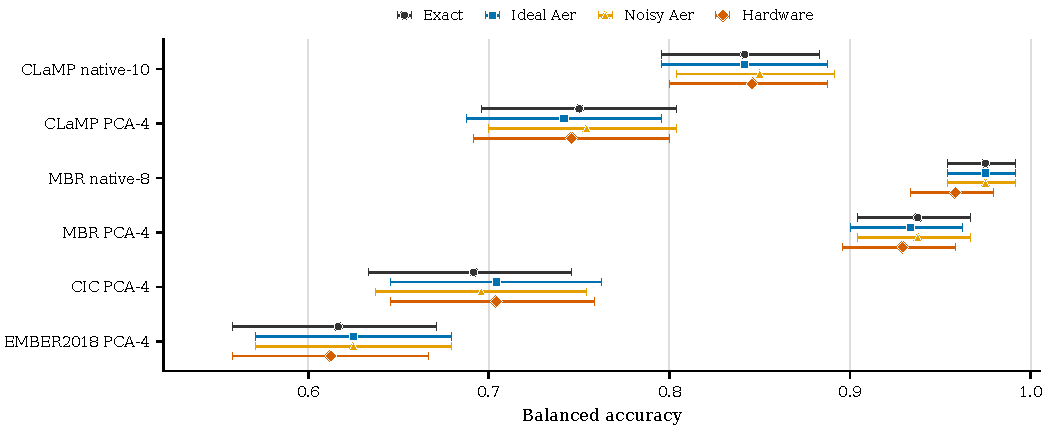
\includegraphics[width=\textwidth]{hardware_results/results/analysis/paper_figure1_execution_performance.pdf}
  \caption{Balanced accuracy across exact, ideal-Aer, noisy-Aer, and IBM hardware execution. Points are means across three held-out splits; bars are 95\% class-stratified bootstrap intervals based on 10,000 replicates and 240 held-out predictions per configuration and environment.}
  \label{fig:execution-performance}
\end{figure*}

Exact balanced accuracy ranged from 0.617 to 0.975 across configurations, compared with 0.625--0.975 for ideal Aer, 0.625--0.975 for noisy Aer, and 0.613--0.958 for hardware. The corresponding hardware ROC AUC values ranged from 0.723 to 0.980. Thus, classification changed little at each step of the execution ladder even when kernel geometry changed more substantially.

\subsection{Kernel Distortion and Circuit Resources}

Relative kernel error increased along the execution ladder (Figure~\ref{fig:kernel-distortion}). Ideal-Aer mean relative error ranged from 0.029 to 0.044, quantifying finite-shot estimation of the ideal transpiled circuits. Noisy-Aer error ranged from 0.069 for EMBER2018 PCA-4 to 0.277 for CLaMP native-10. Hardware error clustered between 0.111 and 0.114 for the four-qubit configurations, compared with 0.441 for MBR native-8 and 0.479 for CLaMP native-10. Hardware kernel correlations with exact kernels were 0.996--0.997 at four qubits, 0.924 at eight qubits, and 0.970 at ten qubits.

\begin{figure*}[t]
  \centering
  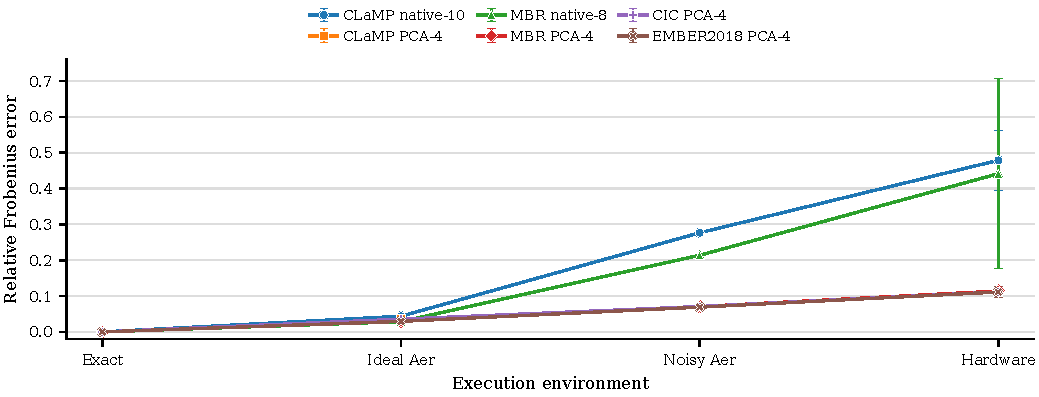
\includegraphics[width=\textwidth]{hardware_results/results/analysis/paper_figure2_kernel_distortion.pdf}
  \caption{Test-kernel relative Frobenius error against the exact statevector kernel. Markers are three-split means and error bars are split standard deviations. Exact kernels define the zero-error reference.}
  \label{fig:kernel-distortion}
\end{figure*}

Across the 18 primary hardware runs, CZ count had a descriptive Pearson correlation of $r=0.857$ (Spearman $\rho=0.812$) with relative kernel error and $r=-0.032$ ($\rho=-0.129$) with hardware-minus-exact balanced accuracy. These values do not isolate a CZ-gate effect. CZ count assumed only three values (22, 54, and 70), the three splits were clustered within configurations, and qubit count, depth, total circuit size, and CZ count increased together. The defensible interpretation is therefore that kernel distortion increased with circuit resource requirements in this experiment, with CZ count strongly associated with error, rather than that CZ gates independently caused the distortion.

PCA reduced circuit cost and hardware distortion but produced a dataset-dependent predictive tradeoff. For CLaMP, reducing the representation from ten to four features lowered circuit depth from 206 to 98 and CZ count from 70 to 22, while hardware balanced accuracy decreased by 10.0 points relative to the native representation. Paired hardware predictions favored native-10 after Holm adjustment ($p=0.0179$). For MBR, PCA reduced width from eight to four qubits and CZ count from 54 to 22; hardware balanced accuracy decreased by 2.9 points, and the adjusted paired-test result was not significant ($p=0.458$).

\subsection{Classical Baselines and Hardware Workload}

The matched classical comparison in Figure~\ref{fig:quantum-classical} did not show a consistent quantum accuracy advantage. RBF SVC matched or exceeded hardware-quantum balanced accuracy on both CLaMP representations, CIC, and EMBER2018; the hardware quantum kernel was descriptively higher on both MBR representations. The linear SVC was below both nonlinear approaches in five configurations, while its 0.621 mean for EMBER2018 was slightly above the 0.613 hardware mean. These comparisons were descriptive and were not part of the prespecified hypothesis-test family.

\begin{figure*}[t]
  \centering
  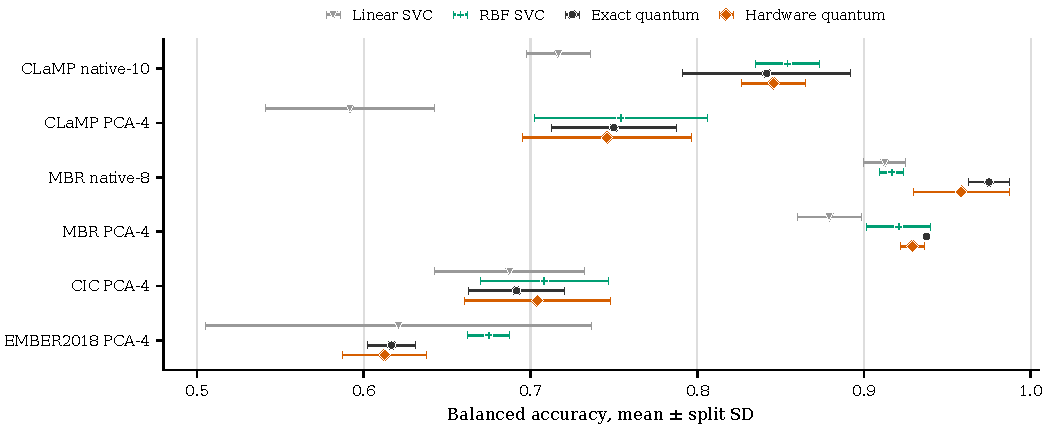
\includegraphics[width=\textwidth]{hardware_results/results/analysis/paper_figure3_quantum_classical.pdf}
  \caption{Matched linear-SVC, RBF-SVC, exact-quantum, and hardware-quantum balanced accuracy. Points are three-split means and bars are split standard deviations. Every classifier used $C=1$ without hyperparameter tuning.}
  \label{fig:quantum-classical}
\end{figure*}

The 18 primary hardware conditions and three prespecified repeat conditions comprised 200,760 kernel evaluations and 102,789,120 circuit shots. All 21 hardware jobs completed without failure or resubmission and totaled 28,189 seconds of IBM-reported QPU usage. This aggregate usage is distinct from the $5.308$--$8.660\,\mu$s single-circuit duration estimates in Table~\ref{tab:circuit-resources}; neither quantity is an end-to-end wall-clock or system-energy measurement.

\section{Discussion}

The principal result was the stability of downstream predictions despite measurable hardware-induced changes in the quantum kernels. Hardware produced substantially greater kernel error than exact or ideal simulation, particularly for the eight- and ten-qubit circuits, yet mean balanced accuracy changed by at most 1.67 percentage points in absolute value. This is notable because numerical kernel fidelity and classification performance were not interchangeable in the experiment. A kernel can differ substantially in aggregate while retaining enough relative structure around the learned SVC decision boundary to produce similar predictions.

The uncertainty analysis limits the strength of that conclusion. The paired confidence intervals include zero, and the McNemar tests found no significant hardware-versus-exact disagreement after multiplicity adjustment. Failure to reject a difference is not evidence of equivalence, however. No practical-equivalence margin was defined before the results were observed, and several paired intervals include changes larger than two percentage points. We therefore interpret the evidence as observed classification stability for these samples, circuits, and hardware runs, not as proof that noisy and exact quantum kernels are generally equivalent.

The circuit-resource results are similarly descriptive. Wider circuits had greater kernel error, and CZ count tracked that error, but width, depth, size, and CZ count were not independently manipulated. Dataset and representation also changed with width. The experiment consequently demonstrates an association between resource-intensive circuits and distortion, not a causal contribution attributable specifically to CZ count.

Feature compression introduced a distinct resource--representation tradeoff. Four-component PCA reduced qubit count, circuit depth, two-qubit gates, and hardware distortion, but it also discarded predictive information. The effect was largest for CLaMP, where PCA-4 reduced hardware balanced accuracy by 10.0 points. MBR showed a smaller 2.9-point reduction. PCA should therefore be presented as reducing resource requirements and distortion with dataset-dependent predictive costs, rather than as preserving accuracy uniformly.

The classical checks likewise do not support a broad quantum-advantage claim. The RBF SVC was competitive with or better than the hardware quantum kernel on several datasets, while the quantum results were descriptively higher on MBR. Because every model used fixed $C=1$ without nested tuning, these results compare matched pipelines rather than optimized classical and quantum methods. Moreover, the experiment did not collect comparable end-to-end latency or system-level energy data, so it provides no evidence of computational or energy advantage.

\subsection{Limitations}

Several constraints bound the findings. Each split used only 80 training and 80 test observations, the balanced class distribution does not reproduce operational malware prevalence, and three repeated holdouts provide limited information about training-sample variability. The study evaluated four datasets but only two native-versus-PCA comparisons, one quantum feature map, two repetitions, linear entanglement, 512 shots, fixed $C=1$, one transpilation per width, one backend, and one short hardware campaign. The noisy-Aer model was frozen from one backend snapshot, while real hardware properties could change during the campaign. Error mitigation was disabled, and the classical baselines were not tuned. Circuit width was coupled to dataset and representation, and no comparable wall-clock or energy measurements were collected.

The datasets also differ in observation type: CLaMP, MBR, and EMBER2018 describe PE files, whereas CIC represents sandbox activity records. Splits were disjoint by source-row identifier and the complete numeric vector used by each model. A post hoc CIC metadata audit nevertheless found two binary hashes recurring across different held-out splits, although no hash appeared in both training and test data within an individual split. CIC therefore does not support file-independent inference across pooled splits. MBR also depends on the provenance and version of its Kaggle source file. The reported values should not be interpreted as full-corpus detector performance or performance under novel malware-family or temporal distribution shift.

\section{Conclusion}

This study compared exact, ideal-Aer, noisy-Aer, and IBM-hardware quantum kernels with matched classical SVCs across four malware datasets. Hardware increasingly distorted the measured kernels as circuit resource requirements grew, but the observed balanced accuracy remained close to exact-kernel performance in all six configurations. Paired uncertainty estimates support describing this as empirical stability under the tested conditions, while not establishing formal equivalence. PCA reduced circuit cost and hardware distortion while causing dataset-dependent losses in predictive performance. Classical RBF models remained competitive, and the experiment did not demonstrate quantum advantage in accuracy, speed, or energy use. The central contribution is instead a reproducible real-hardware observation: substantial numerical kernel distortion need not produce a comparably large change in downstream malware classification.

\subsection{Future Work}

Future evaluations should use larger, hash-, family-, sandbox-session-, and time-grouped samples; nested tuning for classical and quantum models; and repeated execution across devices, calibration windows, feature maps, shot counts, and mitigation settings. Measuring support-vector and margin stability alongside kernel eigenspectra may help identify which distortions alter decisions and which are largely benign. Comparable end-to-end latency and system-level energy measurements are required before assessing resource-based quantum advantage.

An additional direction is a budget-matched comparison between fixed quantum kernels and trainable quantum neural networks. Using the same encodings, splits, shot budgets, and hardware would test whether a learned representation improves predictive performance enough to offset variational optimization noise and whether its inference cost compares favorably with evaluating a new sample against multiple support vectors.

\section{Acknowledgments}

We thank the Monmouth University School of Science Summer Research Program for supporting this project. We also thank Rensselaer Polytechnic Institute for access to its on-campus IBM Quantum System One.

\bibliography{aaai24,paper_additional_references}

\end{document}
